	\newpage
\section{Ogólne określenie wymagań}		%1
%Ogólne określenie wymagań i zakresu programu (Czyli zleceniodawca określa wymagania programu) 




\subsection{Opis działania}  %1.1       

\hspace{0.60cm}Aplikacja na urządzenia mobilne umożliwiająca monitoring dokonań sportowych w dziedzinie biegania. Program ma umożliwić monitorowanie naszej aktywności biegowej. Aplikacja ma zapisywać przede wszystkim czas treningu, dystans, trasę uzyskaną dzięki modułowi GPS oraz intensywność treningu (np. wyliczając średnie tempo, średnią i maksymalną prędkość oraz spalone kalorie). Kożystając z aplikacji mamy mieć możliwość szczegółowej weryfikacji danych treningu, zarówno w trakcie jego trwania jak i po jego zakończeniu. Dodatkowo w podsumowaniu dzięki współpracy programu z GPS-em, można także spawdzić informacje o najniższym i najwyższym punkcie trasy. Szczegółowe statystyki mają pozwolić na analizę postępów i wyciągnięcie wniosków na przyszłość.

Treningi mają być zapisywane w pamięci. Użytkownik ma mieć możliwość zobaczenia statystyk wybranego treningu.

Aplikacja ma za zadanie także motywować nas do ćwiczeń, np. wysyłając nam powiadomienia, w ustalonym przez użytkownika momencie, o tym, że nie odbyliśmy jeszcze treningu.

Poza pomiarami w trakcie treningu, aplikacja ma także liczyć kroki, kiedy działa w tle.






\subsection{Opis wyglądu}  %1.2


\hspace{0.60cm}Na stronie treningu użytkownik w trakcie odbywania treningu, powinien móc odczytać najważniejsze i najbardziej przydatne informacje, takie jak:
\begin{itemize}
	\item Czas trwania aktywności,
	\item Prędkość w danym momencie,
	\item Średnia prędkość,
	\item Dystans,
	\item Spalone kalorie
\end{itemize}

Oprócz tego na stronie treningu Rys. \ref{rys:rysunek001} (s. \pageref{rys:rysunek001}) powinna znajdować się mapa, na~której będzie pokazana aktualna pozycja uzytkownika oraz na której ma być rysowana linią przebyta trasa.

Po zakończonym treningu aplikacja ma pokazać całą przebytą trasę na mapie oraz dać dostęp do szczegółowych statystyk treningu Rys. \ref{rys:rysunek002} (s. \pageref{rys:rysunek002}). Użytkownik ma mieć podgląd na wszystkie możliwe dane.

\begin{figure}[!htb]
	\centering
	\begin{minipage}{.5\textwidth}
		\centering
		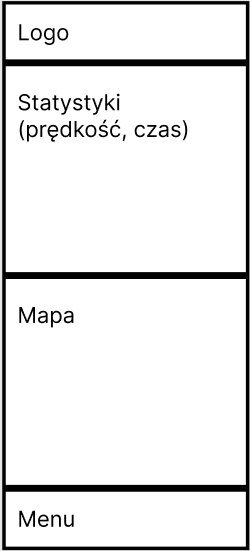
\includegraphics[width=.4\linewidth]{rys/ekran_treningu.png}
		\caption{Ekran treningu}
		\label{rys:rysunek001}
	\end{minipage}%
	\begin{minipage}{.5\textwidth}
		\centering
		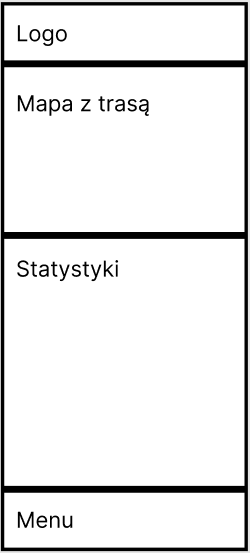
\includegraphics[width=.4\linewidth]{rys/ekran_podsumowania.png}
		\caption{Ekran podsumowania}
		\label{rys:rysunek002}
	\end{minipage}
\end{figure}

Ekran krokomierza Rys. \ref{rys:rysunek003} (s. \pageref{rys:rysunek003}) ma zawierać liczbę zrobionych w~bieżącym dniu kroków. Ekran krokomierza powinien być ekranem głównym, który użytkownik widzi po otwarciu aplikacji, ponieważ zawiera on, które prawdopodobnie są najbardziej interesujące w dany momencie. Oprócz tego w momencie rozpoczęcia treningu na tym ekranie ma~pojawić się dodatkowy licznik pokazujący tylko liczbę kroków zrobionych w trakcie treningu.

\begin{figure}[!htb]
	\centering
	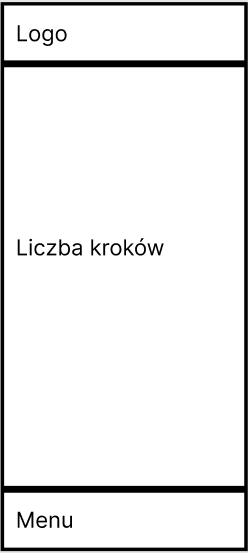
\includegraphics[width=.2\linewidth]{rys/ekran_krokomierza.png}
	\caption{Ekran krokomierza}
	\label{rys:rysunek003}
\end{figure}

Ekran zawierający historię odbytych treningów Rys. \ref{rys:rysunek005} (s. \pageref{rys:rysunek005}) powinien przedstawiać je w~postaci listy. Każdy wpis listy powinien zawierać datę treningu, a~po~naciśnięciu na dany wpis to ma się otworzyć ekran taki sam jak ekran podsumowania po zakończonym treningu, ale tym razem powiniem pokazywać zapisane dane z wybranego treningu. Ekran ustawień Rys. \ref{rys:rysunek006} (s. \pageref{rys:rysunek006}) też powinny być przedstawione w postaci listy. Kliknięcie w wybraną opcję ma otworzyć okienko wpisu zmiany wartości danej opcji.

\begin{figure}[!htb]
	\centering
	\begin{minipage}{.5\textwidth}
		\centering
		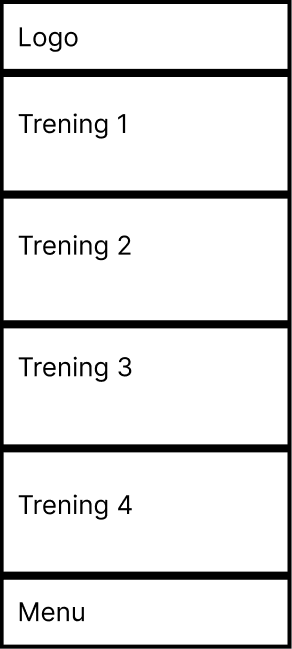
\includegraphics[width=.4\linewidth]{rys/ekran_historii.png}
		\caption{Ekran historii}
		\label{rys:rysunek005}
	\end{minipage}%
	\begin{minipage}{.5\textwidth}
		\centering
		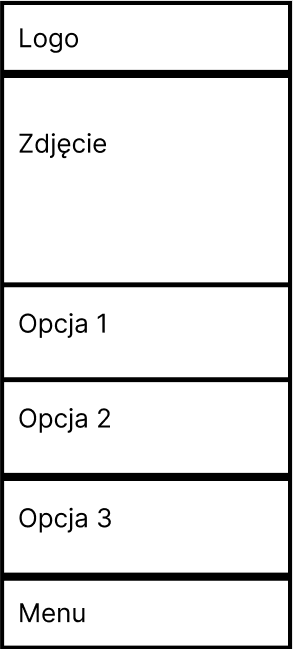
\includegraphics[width=.4\linewidth]{rys/ekran_ustawien.png}
		\caption{Ekran ustawień}
		\label{rys:rysunek006}
	\end{minipage}
\end{figure} 

Aby ułatwić użytkownikom nawigację po aplikacji, na dole ekranu powinno znajdować się intuicyjne menu, które pozwoli na szybkie przejście między poszczególnymi funkcjami. W menu tym powinny znaleźć się przyciski, które po kliknięciu przeniosą użytkownika do ekranu krokomierza, treningu, historii odbytych treningów oraz ekranu ustawień. Dzięki takiemu rozwiązaniu użytkownicy będą mogli łatwo i~szybko dostępować do interesujących ich funkcji, co zwiększy komfort i efektywność korzystania z aplikacji.

Kolorystyka aplikacji powinna być starannie dobrana, aby zapewnić przyjemne i komfortowe doświadczenie użytkownikom. Optymalnym rozwiązaniem będzie zastosowanie odcieni zieleni, które są łagodne dla oczu i nie powodują dyskomfortu podczas dłuższej pracy z aplikacją. Dodatkowo, modernistyczny i nowoczesny wygląd aplikacji pozwoli użytkownikom poczuć, że korzystają z produktu wysokiej jakości, co zwiększy ich zadowolenie i satysfakcję z jej użytkowania. Dlatego ważne jest, aby projekt graficzny był przemyślany i dopracowany, aby spełniał wszystkie wymagania funkcjonalne i estetyczne.